\chapter{Preliminaries and Subproblems}
\label{chap:location_nodes}

\section{Path Selection of Mobile elements}

It is known that controlled MULEs can increase a WSN's lifetime by saving energy. But the problem of planning an optimal path and job schedule is a hard problem in general, known as the Data MULE scheduling problem \cite{dms}. It has three components:
\begin{enumerate}
\item Path selection: which trajectory the data mule follows
\item Speed control: how the data mule changes the speed while moving along the path
\item Job scheduling: from which sensor the data mule collects data at each time point
\end{enumerate}
In this thesis we will focus only on Path selection of the MULEs.

\section{Geometric Disc Covering and Location Nodes}

In the interest of collecting data from sensors in one hop, we propose to cover the sensor field with circular discs of radius equal to the range of the sensors. The centers of these discs are going to be locations where MULEs will pause to collect data from the sensors. We call these positions \emph{location nodes} for convinience. Our path selection heuristic uses location nodes as vertices of a graph embedded on the 2D plane. Ofcourse, we are approximating the communicable region of a sensor to a circular disc, and also assuming that the range of the MULE is greater than that of any sensor (we assume all the sensors are identical in communication range). The centres of these discs are called \emph{location nodes}.

There are two kinds of geometric disc cover problems:

\begin{description}
\item[Geometric minimum disk cover (GMDC)] In this problem, a field of nodes is given, and the aim is to cover all the nodes with minimum number of discs (of given radius) possible. The centers of the discs can lie anywhere on the field.
\item[Geometric discreet unit disc cover (GDUDC)] In this problem, in addition to a field of nodes, a set of points $C$ is also given. The aim is to determine the smallest subset $C'$ of $C$, such that the discs placed at the points in $C'$ cover all the nodes in the field.
\end{description}

We use the problem GMDC here. Compared to GMDC, GDUDC is a much better studied problem. Therefore, we initially planned to get an intermediate solution of GMDC through some heuristic/PTAS, then apply GDUDC problem for a better solution. We tried and failed to implement one solution \cite{carmi} for GDUDC. Therefore, we depend completely upon the following heuristics for disc covering.

There are many heuristics and approximation schemes \cite{shifting} \cite{appScheme} for GMDC already known, any one of which can be used here. Following are four heuristics (JGRD,GRD,SEL,HEX) and one approximation scheme (SHFT) that we tested on sample fields.

\subsection{Preliminaries}
\label{subsec:prelim}

Let $P$ be the set of points to be covered with discs of radius $R$, in the square field $F$. For any two $p_1, p_2 \in P$, there are two $c_1,c_2 \in F$ (called "crosses" for convinience) such that $p_1$ and $p_2$ will lie at the boundary of a disc of radius $R$ placed at either $c_1$ or $c_2$. We consider points $p_1$ and $p_2$ as covered (barely) by any of the two discs above. For any two points $p_1$ and $p_2$ such that distance between $p_1$ and $p_2$ is less than $2R$, there exist two crosses $c_1$ and $c_2$ ($c_1$ and $c_2$ are said to "involve" $p_1$ and $p_2$ for convinience). Let $C$ be the set of all possible crosses in the field $F$.

A set $S$ of disc centres such that they cover all the points in the field $F$ is called a solution of the MGDC problem in the field $F$. Let $S_1$ be such a solution. Then there exists a solution $S_2 \subset C$ such that $|S_1|=|S_2|$.

\subsection{Heuristics}

\begin{description}

\item[OPT] This is the optimum solution algorithm, which uses brute-force to search for the minimum set cover to find the optimum solution. First we make a table of the information regarding which cross (refer \ref{subsec:prelim}) covers which of the sensors. These crosses act like the subsets of the set of all sensors, containing the sensors they cover. We then find the minimum set cover using brute-force. Needless to say, the running time of this algorithm blows up very fast.

\item[HEX] In this heuristic \cite{hex}, first we tile the field with hexagons of sides equal to the radius of the discs to be used (as shown in figure \ref{fig:hex}). A sensor is said to be covered by a hexagon, if it is closer to its center than the center of any other hexagon.
\begin{center}
\begin{figure}[H]
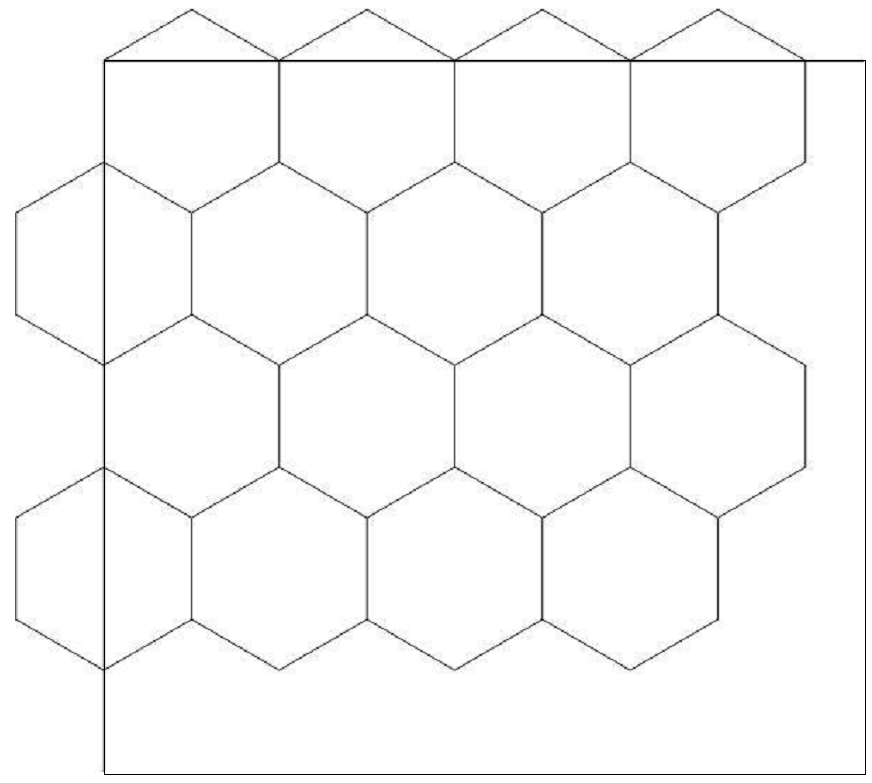
\includegraphics[width=12cm]{figures/hex.png}
\caption{Hexagonal tiling}\label{fig:hex}
\end{figure}
\end{center}

\item[JGRD] This is originally a set cover heuristic \cite{jgreedy}. Consider the set $P$ as the target set to be achieved from the union of smaller subsets, and the discs centered at the crosses in $C$ represent the subsets of points covered by them. Our problem of MGDC then becomes a set cover problem. \cite{jgreedy} gives a greedy heuristic for this.

\item[GRD] (We are not aware of any other work using this heuristic) Let the list of all sensor positions in the field $F$ be $L$. First sort $L$ according to their (x,y) position co-ordinates (first by x co-ordinate and then by y co-ordinate). Starting from the first sensor $p$ in the list, pick the disc which covers maximum number of uncovered sensors and covers $p$ too. To do this, compute all the crosses in $C$ which involve $p$. Place a disc of radius $R$ at each of the crosses, and choose the cross whose disc covers the most number of points. Choose the next uncovered sensor in $L$ and repeat the covering procedure, until all sensors are covered.

\item[SHFT] The shifting strategy from \cite{shifting}. This algorithm takes two input parameters: $l$ (shifting parameter, chosen later) and $D$ (diameter of discs to be used for covering). Let the field be a square of length $W$. First we divide the field into vertical strips of width $l \times D$, as shown in figure \ref{fig:origStrip}. We do disc cover on these vertical strips (explained later) individually (treating them as separate fields. The union of the solutions of all the vertical strips is clearly a solution to the problem. This solution is assigned to $current\_solution$. Now, the whole partition of strips is shifted horizontally, away from the origin, by the amount of $D$ (as shown in figure \ref{fig:shiftStrip}). Again, all the strips are covered with discs (to be explained later how), and the union of the solutions of these shifted vertical strips another solution, assigned to $new\_solution$. If the size of $new\_solution$(the number of discs in the solution) is less than the size of $current\_solution$, the current solution now becomes $new\_solution$. We continue shifting the partition and measuring the solutions thus generated $l-1$ times.

To cover a strip of width $w$, we again apply the shifting strategy. We divide the strip into squares of side $w$ (and maybe a remainder rectangle, in case $W$ leaves a remainder upon dividing with $w$). To cover this sqaure (of size $w \times w$) with discs of diameter D, we use the strategy OPT described above. The shifting of this partition is done by the amount $D$ just like in the original field, and the smallest solution is chosen. The shifting parameter $l$ depends on the time constraint one has regarding the running time of this algorithm. It is chosen in such a way that the problem size in each sqaure (of size $w \times w$) is small enough for the OPT to run in required time constraint.

\begin{figure}[H]

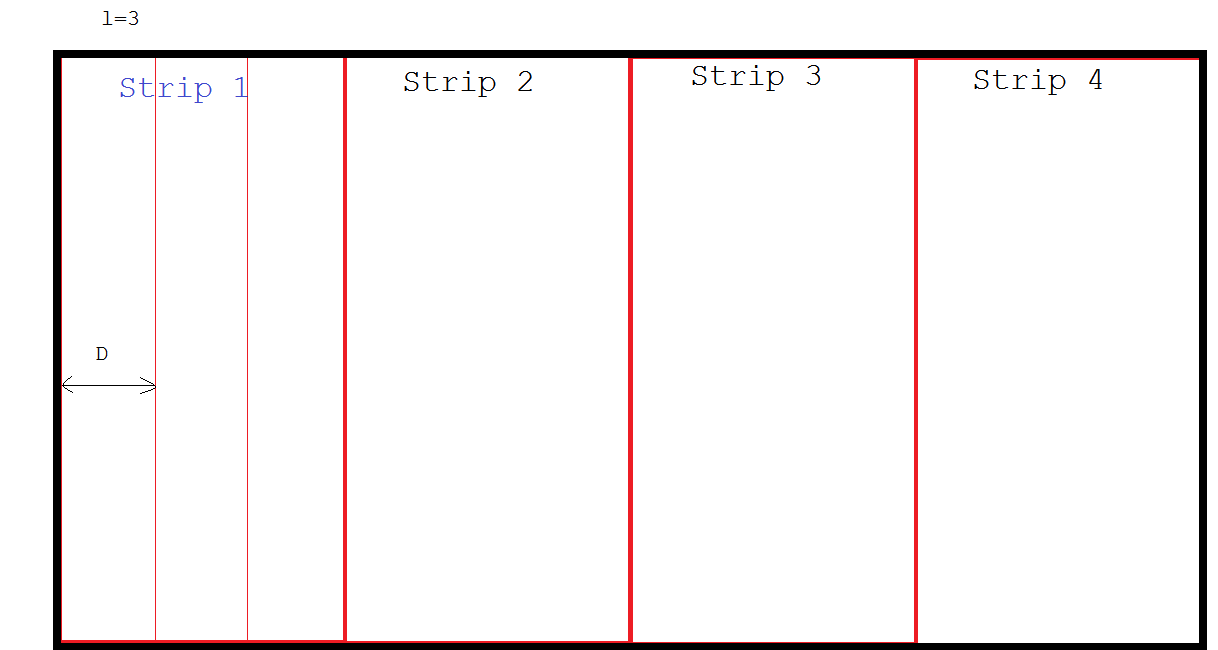
\includegraphics[width=15cm]{figures/beforeShift.png}
\caption{Original division of the field into vertical strips. $l$ is 3 here.} \label{fig:origStrip}

\end{figure}

\begin{figure}[H]

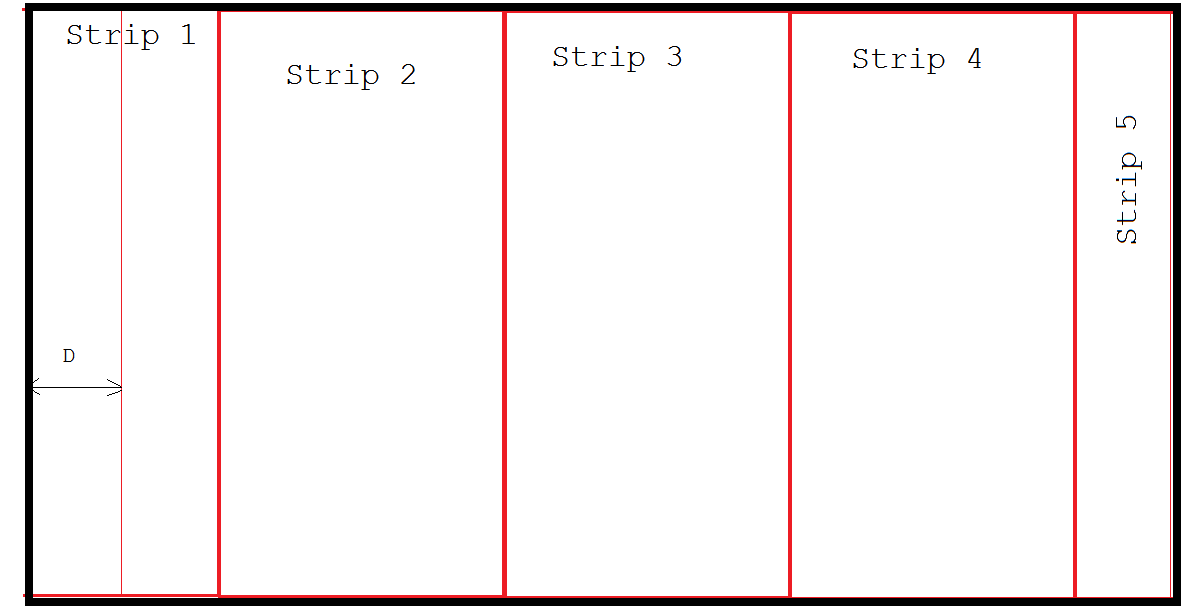
\includegraphics[width=15cm]{figures/afterShift.png}

\caption{After the shift right by the amount $D$}\label{fig:shiftStrip}

\end{figure}

\item[SEL] For any sensor $s$, let $C_s$ be the set of crosses (refer \ref{subsec:prelim}) covering it. Pick the cross which covers the least number of sensors. Keep iterating on the still uncovered sensors, until all the sensors are covered.
\item[RND] Randomly pick crosses until all the sensors are covered. Just for sake of comparision with other heuristics.
\end{description}

\subsection{Results}

The above heuristics and the approximation scheme were tested on a 1000m$\times$1000m field with discs of radius 50m. The number of sensors are increased form 50 to 100 in steps of 10. As we can see, GRD performed the best. Therefore we used GRD of for our implementation.

\begin{figure}[H]
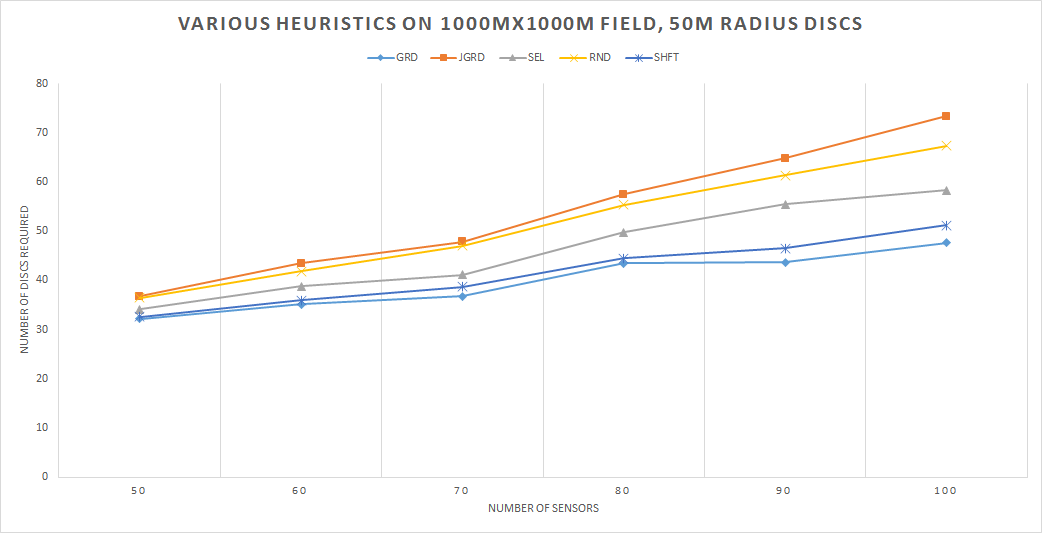
\includegraphics[width=15cm]{discs}
\caption{Results of testing above heuristics and the approximation scheme on a 1000m$\times$1000m field}\label{fig:discResults}
\end{figure}

\section{Euclidean minimum steiner trees}
\begin{definition}[Euclidean minimum Steiner Tree problem]
Given a set $P$ of points in a 2-D plane as input, the output is a network of line segements connecting all of the points in $S$, with the smallest total (Euclidean) length.
\end{definition}
The line segments making the Steiner Tree need just be incident on the points in $S$. This implies that the algorithm is free to use additional points from the plane, if necessary, to produce the smallest total length network. The additional points are called \emph{Steiner points}

For computing Steiner tress, we use the exact solution finder software GeoSteiner ~\cite{geosteiner1} ~\cite{geosteiner2} ~\cite{geosteiner3}. Following figures show a disc cover of 100 sensors in a 1000m$\times$1000m field with discs of radius 50m, and the Steiner trre of the disc centers thus computed.

\begin{figure}[H]
\centering
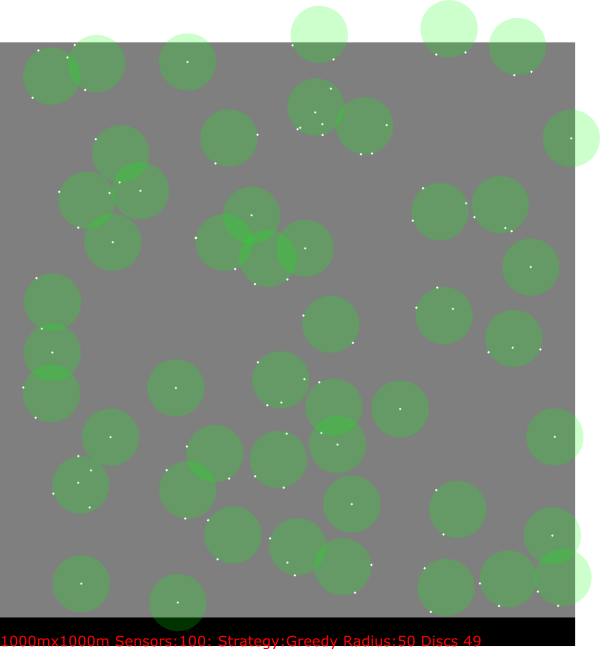
\includegraphics[width=6cm]{figures/disc100.png}
\caption{50m radius disc cover of 100 sensors in 1000x1000 field} \label{fig:disc100}
\medskip
\small
The white dots are sensor positions
\end{figure}

\begin{figure}[H]
\centering
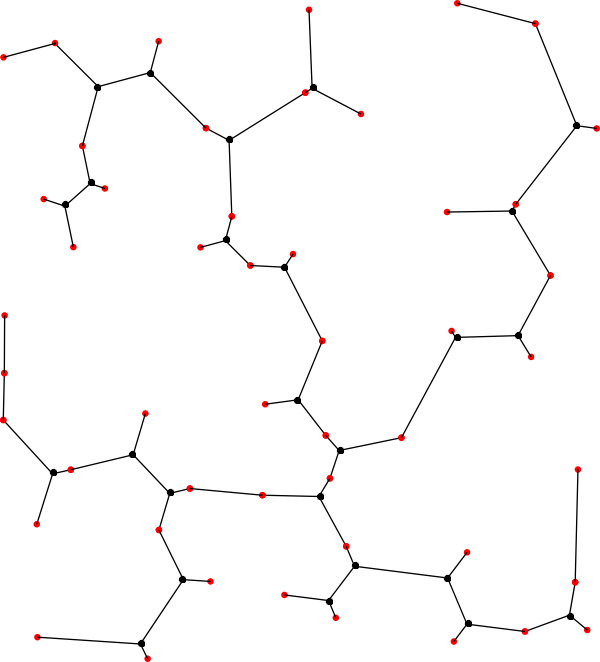
\includegraphics[width=6cm]{figures/steiner100.png}
\caption{The Steiner tree of disc centers of figure \ref{fig:disc100}}
\medskip
\small
The black dots are Steiner points and the red dots are disc centers
\end{figure}